\documentclass[./project-report/src/latex/project-report.tex]{subfiles}

\begin{document}

\maketitle

\clearpage
\section{Design}

\subsection{Introduction}

The following design focuses have been made for the project:

\begin{itemize}
    \item The program will support multiple platforms to run on, including Windows and Linux.
    \item The program will use python3 as its main programming language.
    \item An object-orientated approach is used in the design of the project.
    \item An option will be given to use either a Graphics Card or a CPU to train and test the Artificial Neural Networks.
    \item SysML will be utilised in the design of the architecture and class diagrams
\end{itemize}

\subsection{System Architecture}

The project is architected using object-orientated design principles, it was then implemented in Python. A SysML block diagram \cite{delligatti2013sysml} showing the key 
architectural components is shown in the figure below with detailed SysML class diagrams shown in section \ref{UI-class-diagram}.

As shown in the Figure \ref{fig:system-architecture} the User interacts with the software through a User Interface (UI) which is written in tkinter. The UI classes interface 
with the Model block which contains all the classes necessary for representing the Artificial Neural Network models. As such functional separation is maintained between the 
user interface elements and the Neural Network representation.

\begin{figure}[h!]
\centering
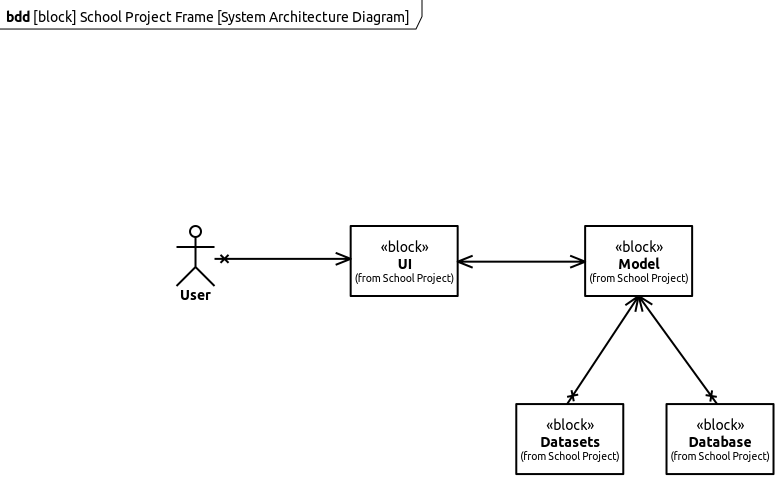
\includegraphics[width=1\textwidth]{./project-report/src/images/system-architecture-diagram.png}
\caption{High level system architecture}
\label{fig:system-architecture}
\end{figure}

\pagebreak

\subsection{Class Diagrams}

\subsubsection{UI Class Diagram}
\label{UI-class-diagram}
The classes utilised to implement the UI are shown in Figure \ref{fig:UI-class-diagram}. As can be seen the School\_Project\_Frame inherits the tk.Frame class - the tkinter 
base class which provides the basic frame functionality. The School\_Project\_Frame then contains a series of UI interaction specific Frames.

\begin{figure}[h!]
\centering
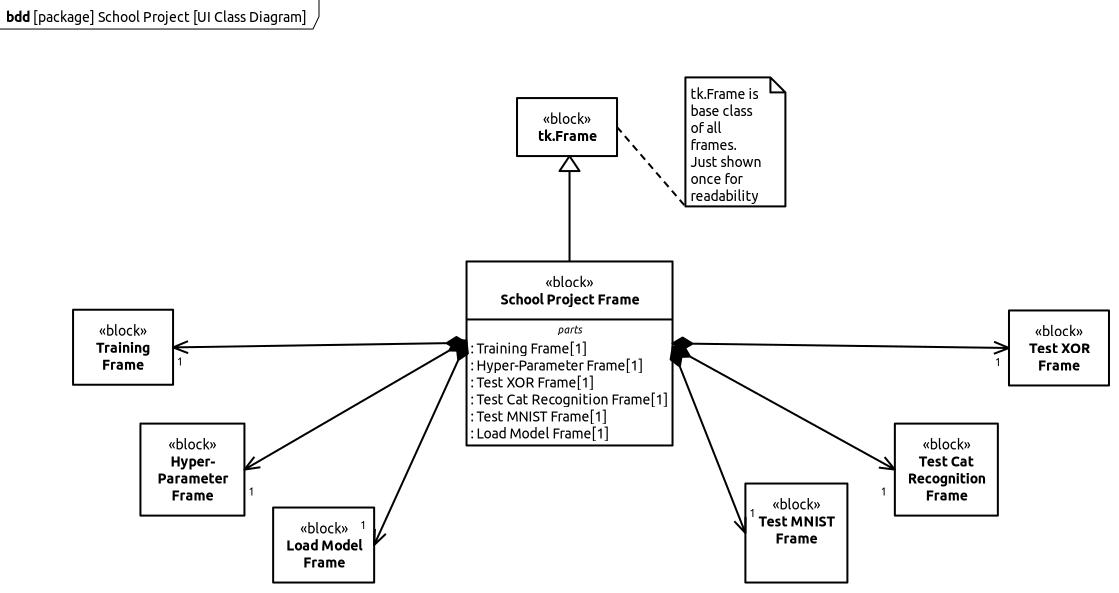
\includegraphics[width=1\textwidth]{./project-report/src/images/ui-class-diagram.png}
\caption{UI SysML Class Diagam}
\label{fig:UI-class-diagram}
\end{figure}

\subsubsection{Model Class Diagram}

The Model class diagram is shown below in figure \ref{fig:model-class-diagram}. An AbstractModel class contains a linked list of FullyConnectedLayer classes which represent 
the layers within the Artificial Neural Network.

\begin{figure}[h!]
\centering
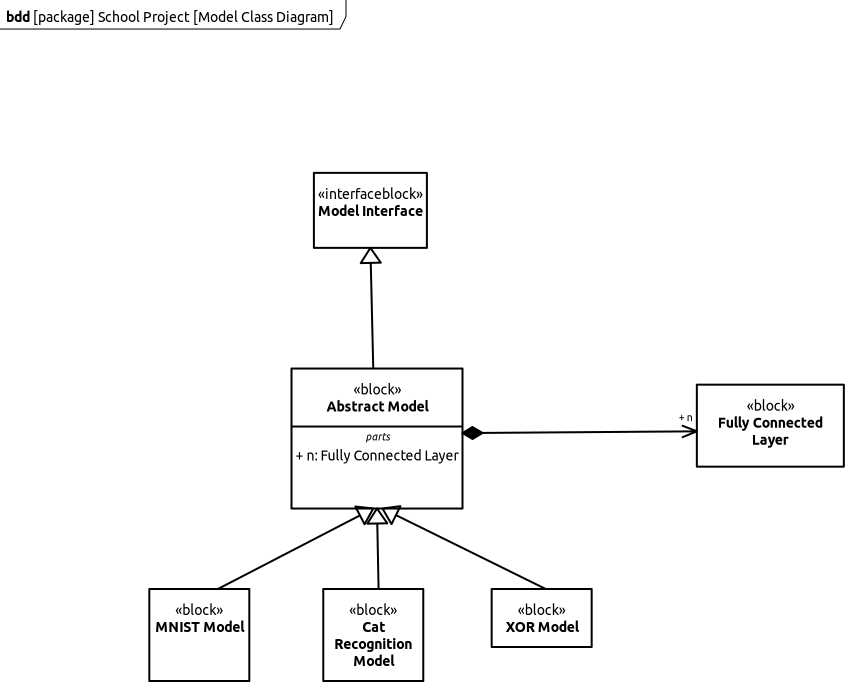
\includegraphics[width=1\textwidth]{./project-report/src/images/model-class-diagram.png}
\caption{Artificial Neural Network and Layers SysML Class Diagram}
\label{fig:model-class-diagram}
\end{figure}

\pagebreak

\subsection{System Flow chart}

The system flow is shown in Figure \ref{fig:system-flow-chart} below. When the program is initialised the Home Frame is first displayed. The left-hand route - 
\textit{Hyper-Parameter Frame} and \textit{Training Frame} - provide the functionality to set hyper-parameters and train a new model. This model can be saved and loaded, 
following the right-hand route, if desired before entering the \textit{Testing Frame} where the model can be applied to testing data and the model performance assessed. The 
ability to save models is important as it allows for model training on a computer with a GPU and utilisation on a non-GPU-accelerated computer. This allowed an efficient build test cycle as I could build models on a desk-based, GPU accelerated PC, and undertake testing / demonstration on a laptop.

\begin{figure}[h!]
\centering
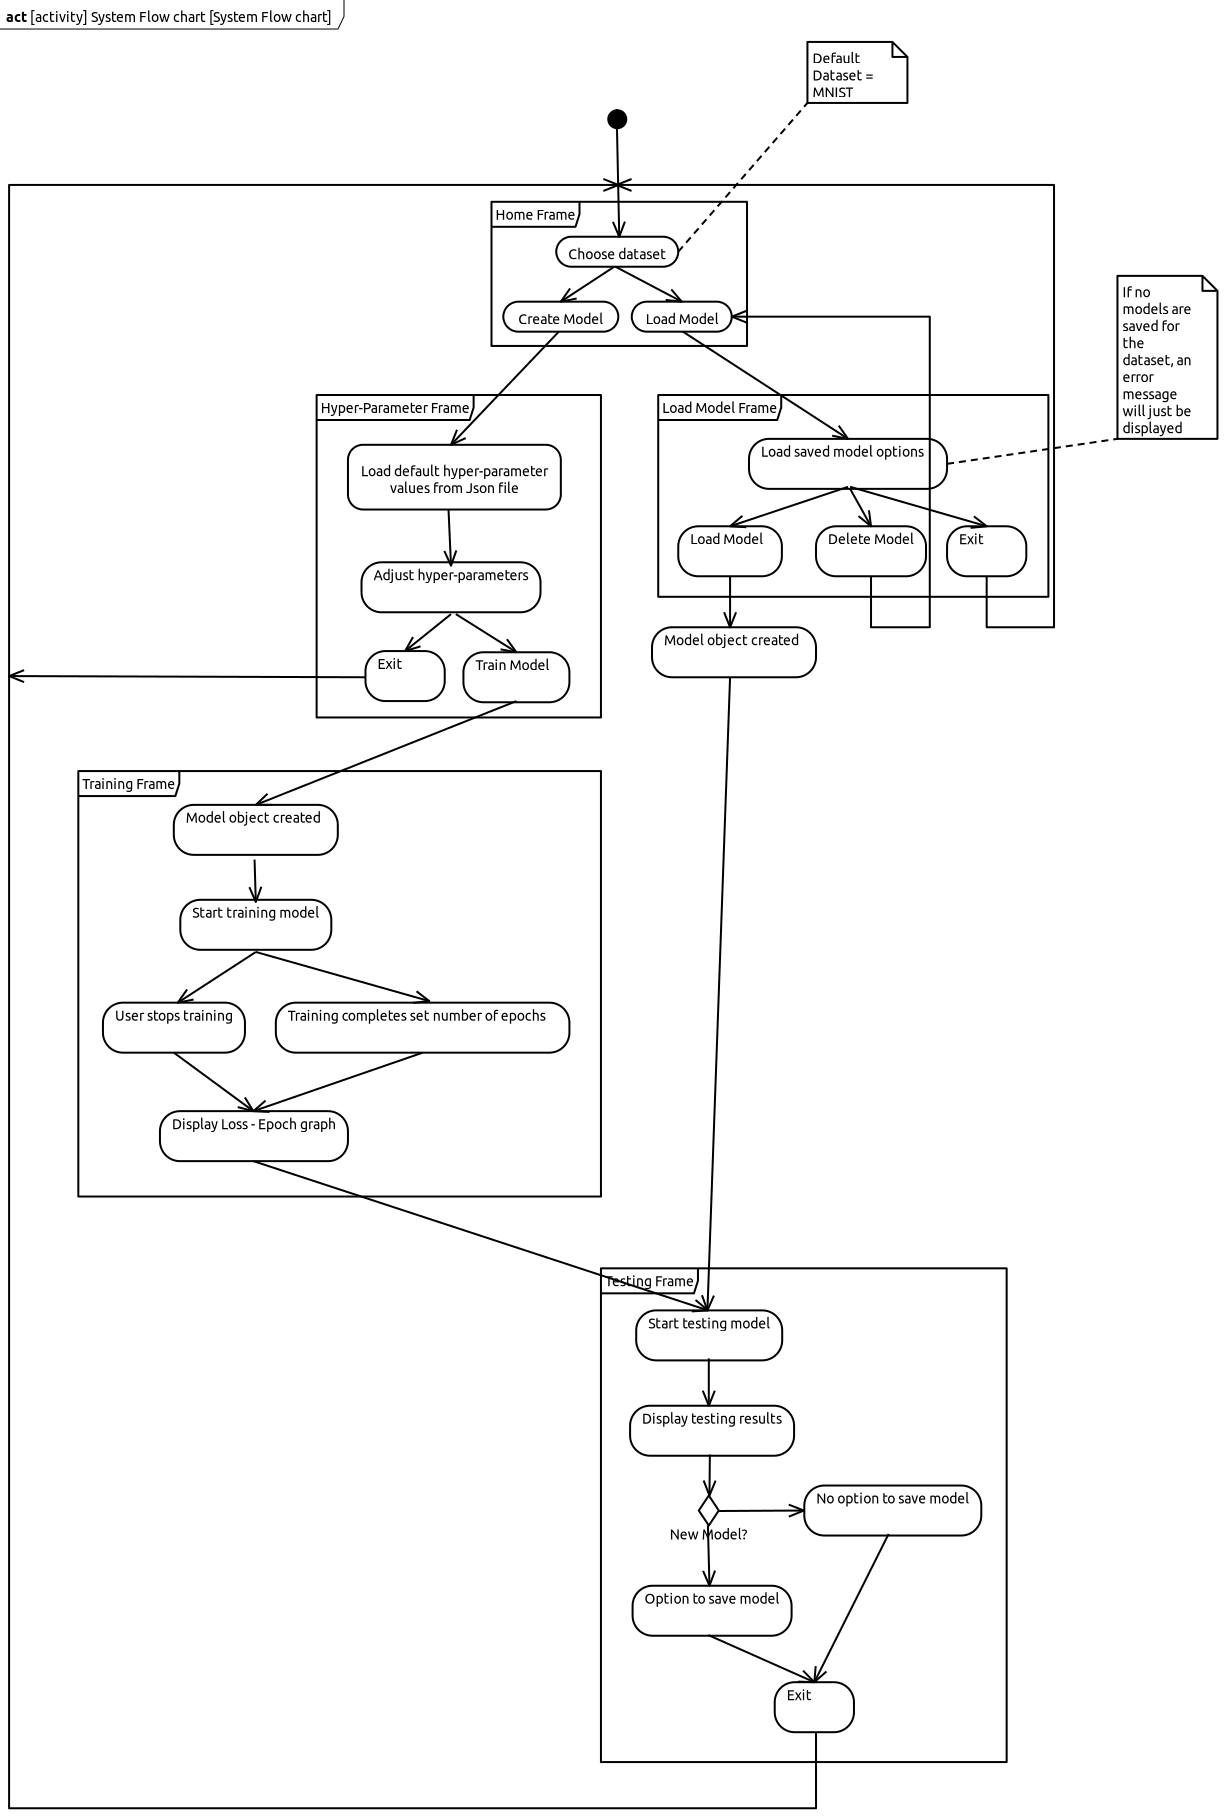
\includegraphics[width=1\textwidth]{./project-report/src/images/system-flow-chart.png}
\caption{System flow chart}
\label{fig:system-flow-chart}
\end{figure}

\subsection{Algorithm implementation}

The detail of algorithms underpinning the Artifical Neural Network are outlined in section \ref{sec:ann-theory}. To implement the algorithm within the project each layer 
within the Artificial Neural Network is represented as an instance of a \textit{FullyConnectedLayer} class each of which:

\begin{itemize}
    \item Contains a weight and bias matrix.
	\item Has a \textit{transfer\_function} which be selected by the user to be either Sigmoid or ReLu but can be easily extended to other functions.
    \item Has a \textit{forward\_propagation} function which takes an input matrix which it then multiplies by the weight matrix and sums the result with the bias matrix, this 
		  is then put through the \textit{transfer\_function}.
    \item Has a \textit{backward\_propagation} function which passes the loss with respect to each layers output allowing adjustment of the weights and biases.
\end{itemize}

Each \textit{FullyConnectedLayer} class is held within a doubly linked list contained within the \textit{Abstract Model Class}, which is a parent class of the 
data-specific classes \textit{MNIST Model}, \textit{Cat Recognition Model} and \textit{XOR Model}. The use of a doubly linked list allows for a user defined number of hidden 
layers from 0 upwards and allows easy propagation of the list.

The algorithm to train the Artificial Neural Network iterates over a user-defined number of epochs. Each epoch starts with the presentation of data to the input layer. The 
doubly linked list of layers is then traversed calling the \textit{forward\_propagation} function on each. When the output layer is reached the derivative of the 
\textit{Log-Loss} function is calculated alongside the absolute \textit{Loss} for debugging and learning rate plotting. 

Following the calculation of the derivative of the \textit{Log-Loss} function, the doubly linked list is then iterated in reverse back through the layers calculating the loss 
with respect to the weights and biases of each layer. This process is then used to adjust the weights and biases in each layer using the specified learning rate in an attempt 
to reduce the loss value.

\subsection{Data Structures, Techniques and File Structures used}

\subsubsection{Data structures}

The following data structures are utilised in implementing the Artificial Neural Network:

\begin{itemize}
    \item Standard lists for storing data, for example storing the shape of the Artificial Neural Network's layers.
    \item Tuples where tuple unpacking is useful, such as returning multiple values from methods.
    \item Dictionaries for loading the default hyper-parameter values from a JSON file.
    \item Matrices to represent the layers and allow for a varied number of neurons in each layer. To represent the Matrices I will use both numpy arrays and cupy 
          arrays.
    \item A Doubly linked list to represent the Artificial Neural Network, where each node is a layer of the network. This allows traversing both forwards and 
          backwards through the network, as well as storing the first and last layer to start forward and backward propagation respectively.
\end{itemize}

\subsubsection{Techniques}

Some techniques used include:

\begin{itemize}
    \item Object-oriented design including inheritance, abstract classes and interfaces
    \item Encapsulation
    \item Decorators to wrap functions and modify behaviour
    \item tkinter for user interface design
    \item SQL for database access
\end{itemize}

\subsubsection{File Structure}

I have used the following file structures to store necessary data for the program:

\begin{itemize}
	\item A JSON file \cite{w3json} for storing the default hyper-parameters for creating a new model for each dataset.
	\item Image dataset files are stored in either a compressed archive file (such as .pkl.gz files) or of the Hierarchical Data Format (such as .h5) for storing large 
		  datasets with fast retrieval.
	\item Weights and biases of saved models are stored as numpy arrays in .npz files (a zipped archive file format) in a 'saved-models' directory, which allows compatibility 
		  with the standard numpy library.
\end{itemize}

\pagebreak

\subsection{Database Design}

The following Relational database design is used for saving models, where the dataset, name and features of the saved model (including the location of the 
saved models' weights and biases and the saved models' hyper-parameters) are saved. The Model\_ID field is the primary key.

\begin{figure}[h!]
\centering
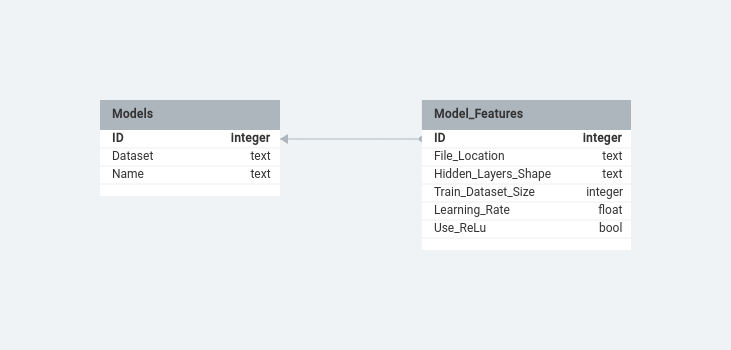
\includegraphics[width=1\textwidth]{./project-report/src/images/database-design.png}
\caption{Database design}
\label{fig:database-design}
\end{figure}

The following unique constraint is also used so that each dataset can not have more than one model with the same name:

\begin{minted}{sql}
UNIQUE (Dataset, Name)
\end{minted}

The following constraint is applied to ensure no attribute is left empty:

\begin{minted}{sql}
NOT NULL
\end{minted}

\subsection{Queries}

Below are some example queries used for interacting with the database:

\begin{itemize}
    \item Query the names of all saved models for a dataset:
    \begin{minted}{sql}
    SELECT Name FROM Models WHERE Dataset=?;
    \end{minted}
    \item Query the file location of a saved model:
    \begin{minted}{sql}
    SELECT File_Location FROM Models WHERE Dataset=? AND Name=?;
    \end{minted}
    \item Query the features of a saved model:
    \begin{minted}{sql}
    SELECT * FROM Models WHERE Dataset=? AND Name=?;
    \end{minted}
\end{itemize}

\subsection{Human-Computer Interaction}

Below are the designs of each tkinter frame in the User Interface. The flow of the frames is described in Figure \ref{fig:system-flow-chart}. The final implementation of the 
frames is shown in the technical solution section.

\begin{itemize}
    \item The home Frame design which acts as the entry point to the program, the implemented version is shown in Figure \ref{fig:home-frame-impl}.
        \begin{figure}[h!]
        \centering
        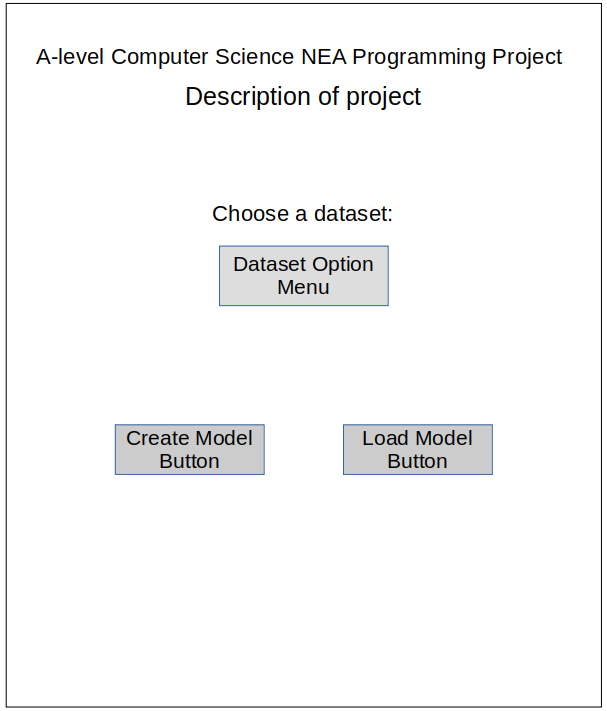
\includegraphics[width=0.7\textwidth]{./project-report/src/images/home-frame-design.png}
        \caption{Home frame design - the entry point to the program}
        \label{fig:home-frame-design}
        \end{figure}

    \pagebreak

    \item Hyper-Parameter Frame design which allows setting of the Hyper-parameters, the implemented version is shown in Figure \ref{fig:hyper-parameter-frame}.
        \begin{figure}[h!]
        \centering
        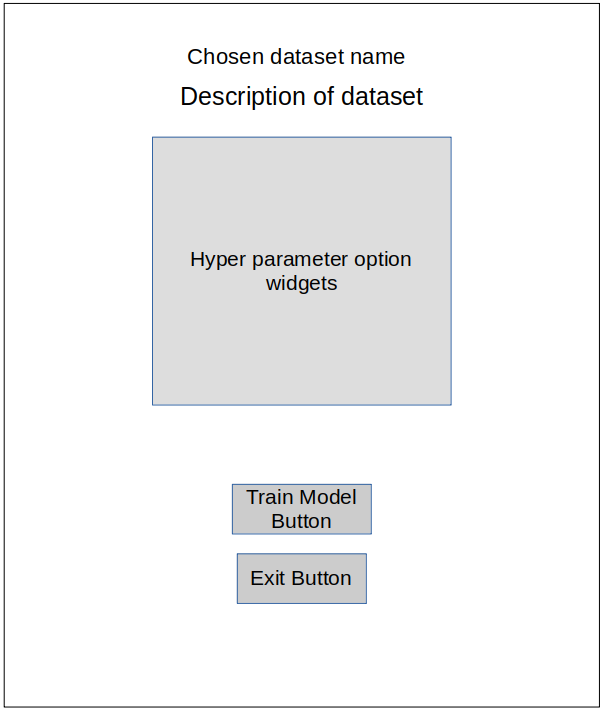
\includegraphics[width=0.7\textwidth]{./project-report/src/images/hyper-parameter-frame-design.png}
        \caption{Hyper-Parameter Frame design which allows setting of parameters}
        \label{fig:hyper-parameter-frame-design}
        \end{figure}

    \pagebreak

    \item Training Frame design: 
        \begin{itemize}
            \item During training, the following is displayed on the Training Frame, the implemented version is shown in Figure \ref{fig:training-frame-1-impl}
                \begin{figure}[h!]
                \centering
                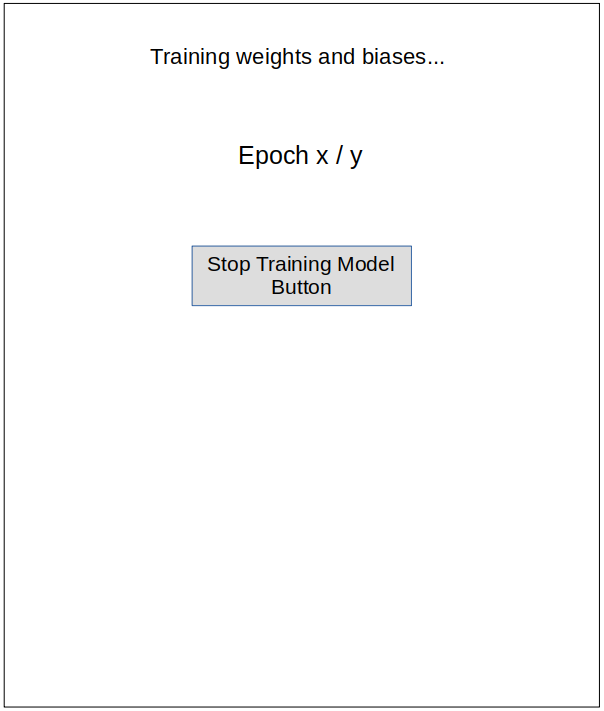
\includegraphics[width=0.7\textwidth]{./project-report/src/images/training-frame-1-design.png}
                \caption{Training frame layout during training}
                \label{fig:training-frame-1-design}
                \end{figure}

            \pagebreak

            \item Once training has finished, the following is displayed on the Training Frame, the implemented version is shown in Figure \ref{fig:training-frame-2-impl}.
                \begin{figure}[h!]
                \centering
                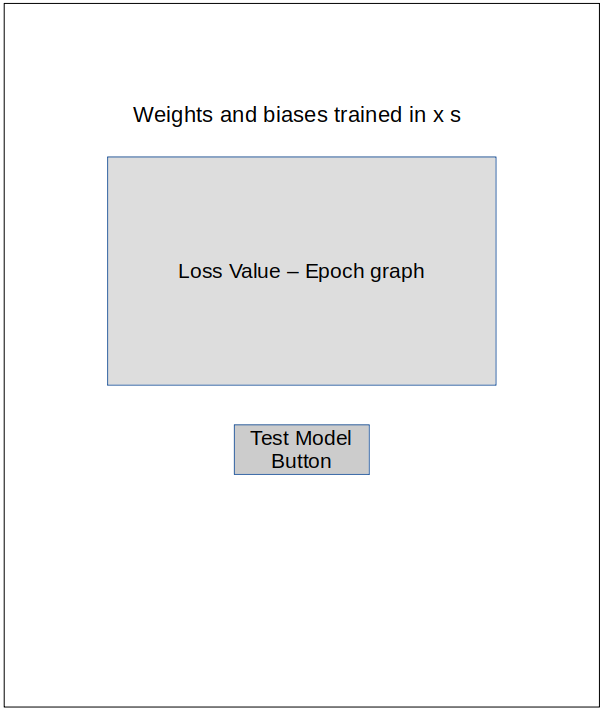
\includegraphics[width=0.7\textwidth]{./project-report/src/images/training-frame-2-design.png}
                \caption{Training frame layout after training}
                \label{fig:training-frame-2-design}
                \end{figure}
            \end{itemize}

    \pagebreak

    \item Load Model Frame design, the implemented version is shown in Figure \ref{fig:load-model-frame-impl}.
        \begin{figure}[h!]
        \centering
        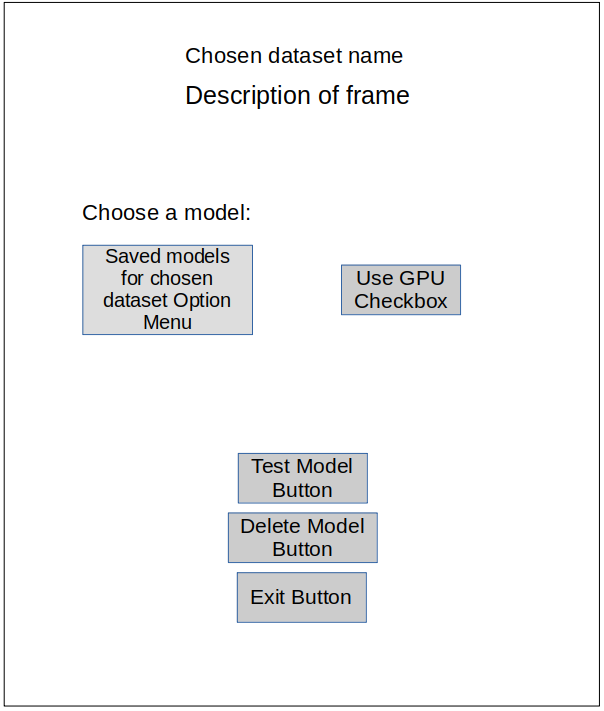
\includegraphics[width=0.7\textwidth]{./project-report/src/images/load-model-frame-design.png}
        \caption{Load model frame design}
        \label{fig:load-model-frame-design}
        \end{figure}
    
    \pagebreak
    
    \item Test Frame design, the implemented version is shown in Figure \ref{fig:test-frame-impl}.
        \begin{figure}[h!]
        \centering
        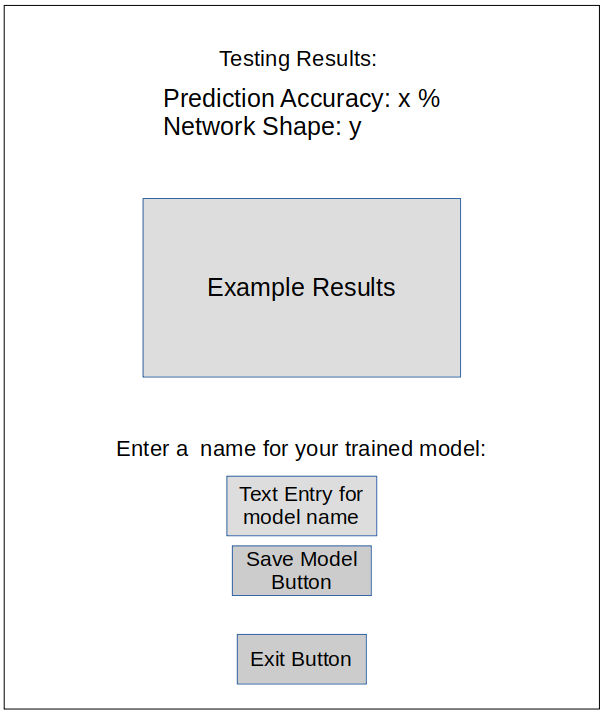
\includegraphics[width=0.7\textwidth]{./project-report/src/images/testing-frame-design.png}
        \caption{Test frame design}
        \label{fig:testing-frame-design}
        \end{figure}
\end{itemize}

\subsection{Hardware Design}

To allow for faster training of an Artificial Neural Network, I gave the option to use a Graphics Card to train the Artificial Neural Network where available. I also gave the 
option to load pretrained weights to run on less computationally powerful hardware using just the CPU as standard. This was implemented by using the CuPy library.

\subsection{Workflow and source control}

Git and GitHub were used to manage the workflow and provide source control as the project was developed. In particular the following features were utilised:

\begin{itemize}
    \item Commits and branches for adding features and fixing bugs separately.
    \item Using GitHub to back up the project as a repository.
    \item Automated testing on GitHub after each pushed commit.
    \item Providing the necessary instructions and information for the installation and usage of this project, as well as creating releases of the project with new patches.
\end{itemize}

\end{document}
